\section{Анализ задания}
В рамках курса было необходимо разработать приложение для распределенных вычислительных систем. Приложение должно удовлетворять требованиям открытости, масштабируемости и прозрачности, применять технологии EJB и JPA и использовать Web-интерфейс для взаимодействия с пользователем.

Было решено разработать информационную систему для научного журнала.

\subsection{Модель предметной области}

\begin{figure}[H]
\centering
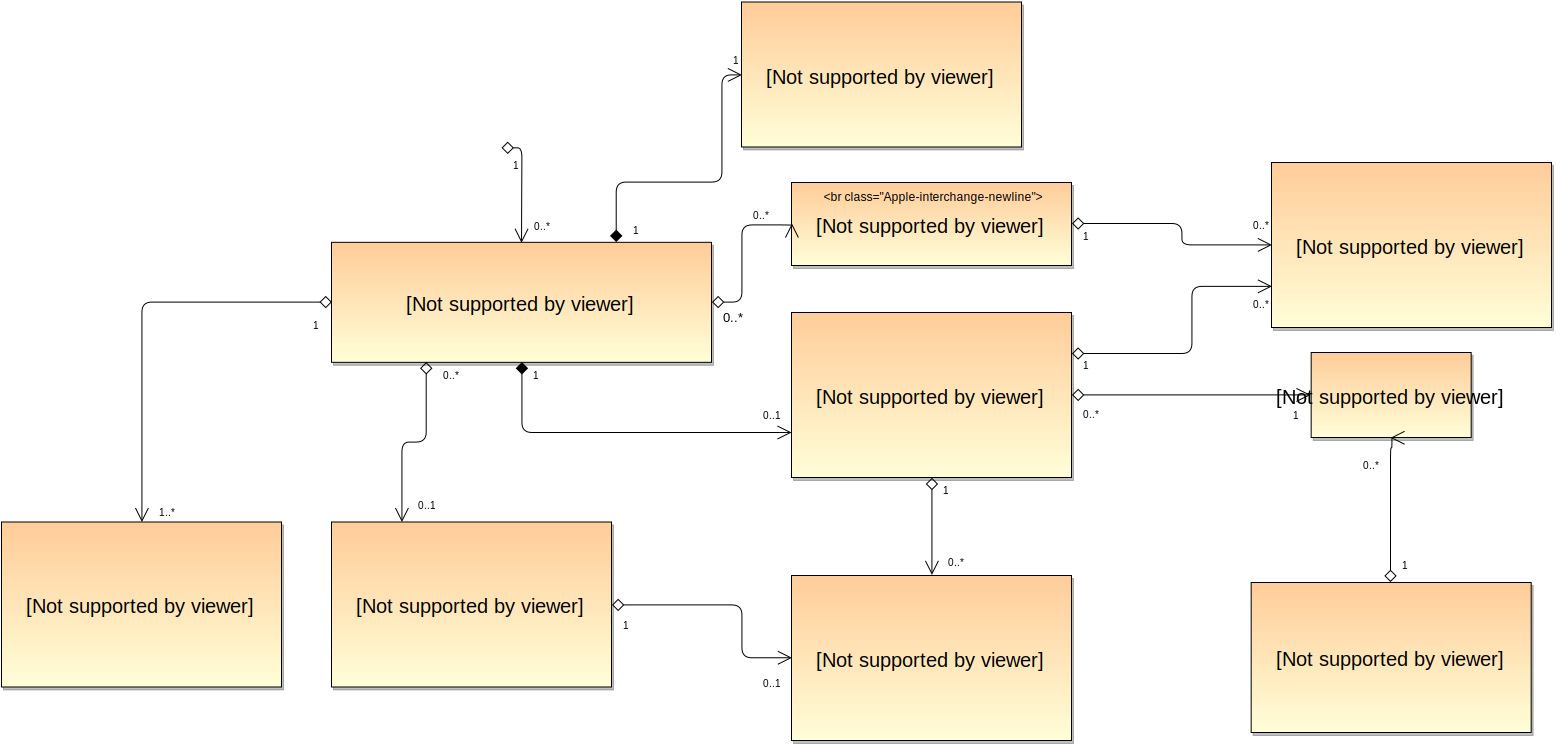
\includegraphics[width=\textwidth]{ClassDiagram.pdf}
\caption{Модель предметной области}
\end{figure}

\subsection{Роли}

В проекте выделено 3 роли: исследователь, редакция и рецензент:

\begin{itemize}
\item Исследователь

\begin{itemize}
\item Разрабатывает научную тему
\item Пишет статью по ней
\item Принимает замечания по ней
\item \textit{Цель:} Чтобы его статья была опубликована в журнале
\end{itemize}
\item Рецензент

\begin{itemize}
\item Выбирается редакцией
\item Получает статьи для просмотра
\item Дает оценку статье (стоит ли принимать для публикации)
\item Высказывает замечания, возникшие при прочтении статьи
\item \textit{Цель:} Выбрать подходящие статьи
\end{itemize}
\item Редакция

\begin{itemize}
\item Принимает статьи
\item Устанавливает правила принятия статей
\item Подбирает рецензентов
\item Связывает рецензентов и авторов
\item Корректирует статьи, если необходимо
\item Издает журнал с помощью типографии
\item \textit{Цель:} Принять качественные статьи, заработать на продаже журналов
\end{itemize}
\end{itemize}

\section{Варианты использования}

\subsection{Написание и подача статьи}

\begin{enumerate}
\item Исследователь запрашивает веб-страницу, предназначенную для добавления новой публикации.
\item Система запрашивает из БД список исследователей, и помещает их имена на веб-страницу в виде выпадающего списка, с возможностью выбора одного из них.\\ Также система запрашивает из БД список всех публикаций, и для каждой публикации помещает на страницу её заголовок, реферат и содержимое
\item Исследователь на странице в выпадающем списке выбирает своё имя и нажимает кнопку <<Отправить>>.
\item Система фиксирует у себя имя текущего исследователя и перерисовывает страницу, добавляя на неё имя исследователя.
\item Автор заполняет на странице поля <<Заголовок>>, <<Реферат>> (Abstract) и <<Содержимое статьи>> (Content). После заполнения всех полей автор нажимает кнопку <<Отправить>>.
\item Система создает объект типа <<Статья>> (Paper), заполняя его присланными пользователем данными. В качестве автора указывается текущий исследователь. После этого система создает объект типа <<Подача>> (Submission), указывая в качестве его атрибута только что созданную статью. Оба объекта помещаются в БД.
\item Система перерисовывает страницу, в списке статей появляется только что добавленная статья
\end{enumerate}

\subsection{Проверка статьи редактором журнала}

\begin{enumerate}
\item Редактор запрашивает веб-страницу, предназначенную для добавления новой оценки.
\item Система запрашивает из БД список всех не просмотренных редакцией публикаций, и для каждой публикации помещает на страницу её заголовок, реферат и содержимое. На страницу рядом с каждой статьей в списке помещается набор кнопок для выставления решения.
\item Редактор просматривает статьи и решает, что одна из статей соответствует тематике журнала и удовлетворяет правилам оформления. Редактор нажимает кнопку <<Одобрить>> около статьи в списке.
  \begin{itemize}
  \item
    Альтернатива: Редакция отказывает в приеме статьи по причине недоработок в статье (например, проблемах с форматированием). Редактор в текстовом поле указывает список замечаний, который будет передан автору, и нажимает кнопку <<Отправить на доработку>>
  \item
    Альтернатива: Редакция отказывает в приеме по причине несоответствия тематике журнала. Редактор в текстовом поле указывает список замечаний, который будет передан автору, и нажимает кнопку <<Статья для другого журнала>>.
  \end{itemize}
\item Система создает объект типа <<Оценка редактора>> (EditorialReview), указывая в нем оценку и комментарий редактора. Система получает из БД объект <<Подача>> (Submission) для указанной статьи и добавляет в него объект <<Оценка редактора>>. Также у объекта подачи устанавливается состояние, соответствующее выбору редактора (Одобрить/Доработать/Перенаправить).
\item Система перерисовывает страницу, из списка статей исчезает только что оцененная статья.
\end{enumerate}

\subsection{Рецензирование}

\begin{enumerate}
\item Рецензент запрашивает веб-страницу, предназначенную для добавления новой рецензии.
\item Система запрашивает из БД список рецензентов, и помещает их имена на веб-страницу в виде выпадающего списка, с возможностью выбора одного из них.\\ Также система запрашивает из БД список всех одобренных редакцией публикаций, и для каждой публикации помещает на страницу её заголовок, реферат и содержимое. На страницу рядом с каждой статьей в списке помещается набор кнопок для выставления решения.
\item Рецензент на странице в выпадающем списке выбирает своё имя и нажимает кнопку <<Отправить>>.
\item Система фиксирует у себя имя текущего рецензента и перерисовывает страницу, добавляя на неё имя исследователя.
\item
  Рецензент просматривает статьи и решает, что одна из статей достойна публикации в журнале. В поле <<Замечания>> на странице сайта он указывает свою рецензию. Рецензент нажимает кнопку <<Accept>>, статья отмечается в системе как принятая и исчезает из списка не просмотренных.
  
  \begin{itemize}
  \item
    Альтернатива: Рецензент имеет замечания к статье, но допускает её для публикации (Neutral). В поле <<Замечания>> на странице сайта он указывает свою рецензию. Рецензент нажимает кнопку <<Neutral>>.
  \item
    Альтернатива: Рецензент имеет замечания к статье и не допускает её для публикации (Reject). В поле <<Замечания>> на странице сайта он указывает свою рецензию. Рецензент нажимает кнопку <<Reject>>.
  \end{itemize}
\item Система создает объект типа <<Оценка рецензента>> (ReviewerRemark), указывая в нем оценку и комментарий рецензента. Система получает из БД объект <<Подача>> (Submission) для указанной статьи и в качестве атрибута <<Рецензия>> указывает у него только что созданный объект. Также у объекта подачи устанавливается состояние, соответствующее выбору рецензента (Accept, Neutral, Reject).
\item Система перерисовывает страницу, из списка статей исчезает только что оцененная статья.
\end{enumerate}

\subsection{Диаграмма вариантов использования}

\begin{figure}[H]
\centering
\includegraphics[width=\textwidth]{UseCases.pdf}
\caption{Диаграмма вариантов использования}
\end{figure}

\subsection{Диаграмма последовательностей}

\subsubsection{Получение списка статей}

\begin{figure}[H]
\centering
\includegraphics[width=\textwidth]{seq_papers.png}
\caption{}
\end{figure}

\subsubsection{Подача статей}

\begin{figure}[H]
\centering
\includegraphics[width=\textwidth]{seq_researcher.png}
\caption{}
\end{figure}

\subsubsection{Редакция}

\begin{figure}[H]
\centering
\includegraphics[width=\textwidth]{seq_editor.png}
\caption{}
\end{figure}

\subsubsection{Рецензирование}

\begin{figure}[H]
\centering
\includegraphics[width=\textwidth]{seq_reviewer.png}
\caption{}
\end{figure}

\section{Реализация задания с помощью технологии EJB}

\subsection{Объектно-ориентированное проектирование с учётом особенностей технологии}

Ниже приведена диаграмма классов для пакета objects, в котором содержатся классы, соответствующие сущностям предметной области. Альтернативы из вариантов использования представлены в приложении в виде перечислений Decision и Mark.

Для отслеживания состояния статьи используется перечисление State, имеющее варианты для каждого этапа обработки статьи.

\begin{figure}[H]
\centering
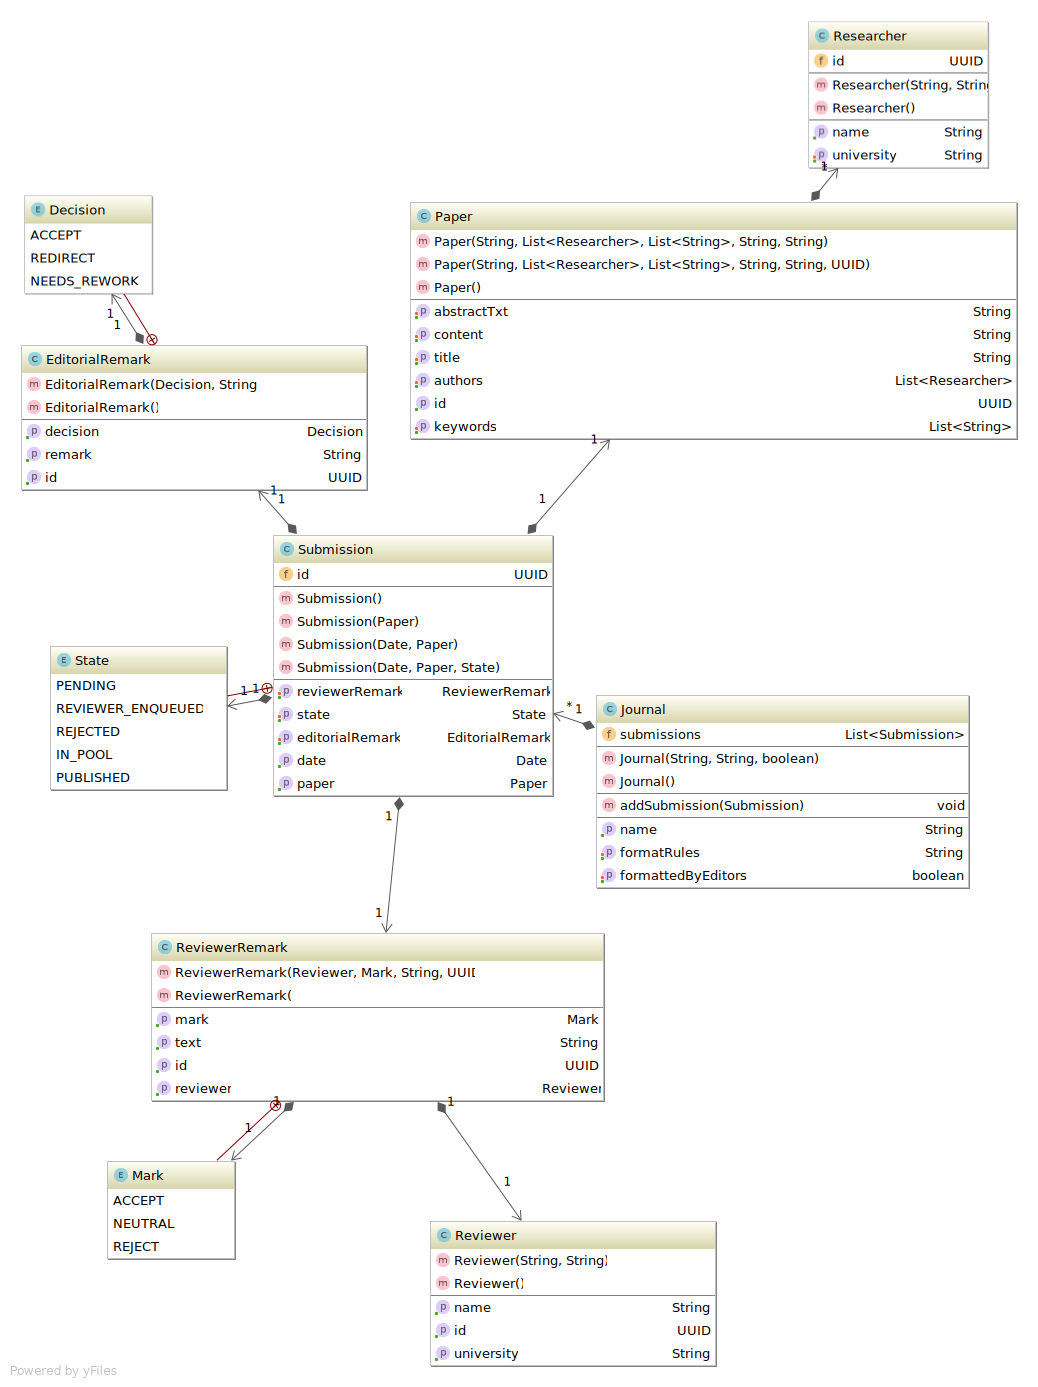
\includegraphics[width=\textwidth]{diagram.pdf}
\caption{Диаграмма класса для пакета objects}
\end{figure}

Ниже приведена диаграмма классов для пакетов services и repository, содержащих различные сервисы, используемые в приложении.

\begin{figure}[H]
\centering
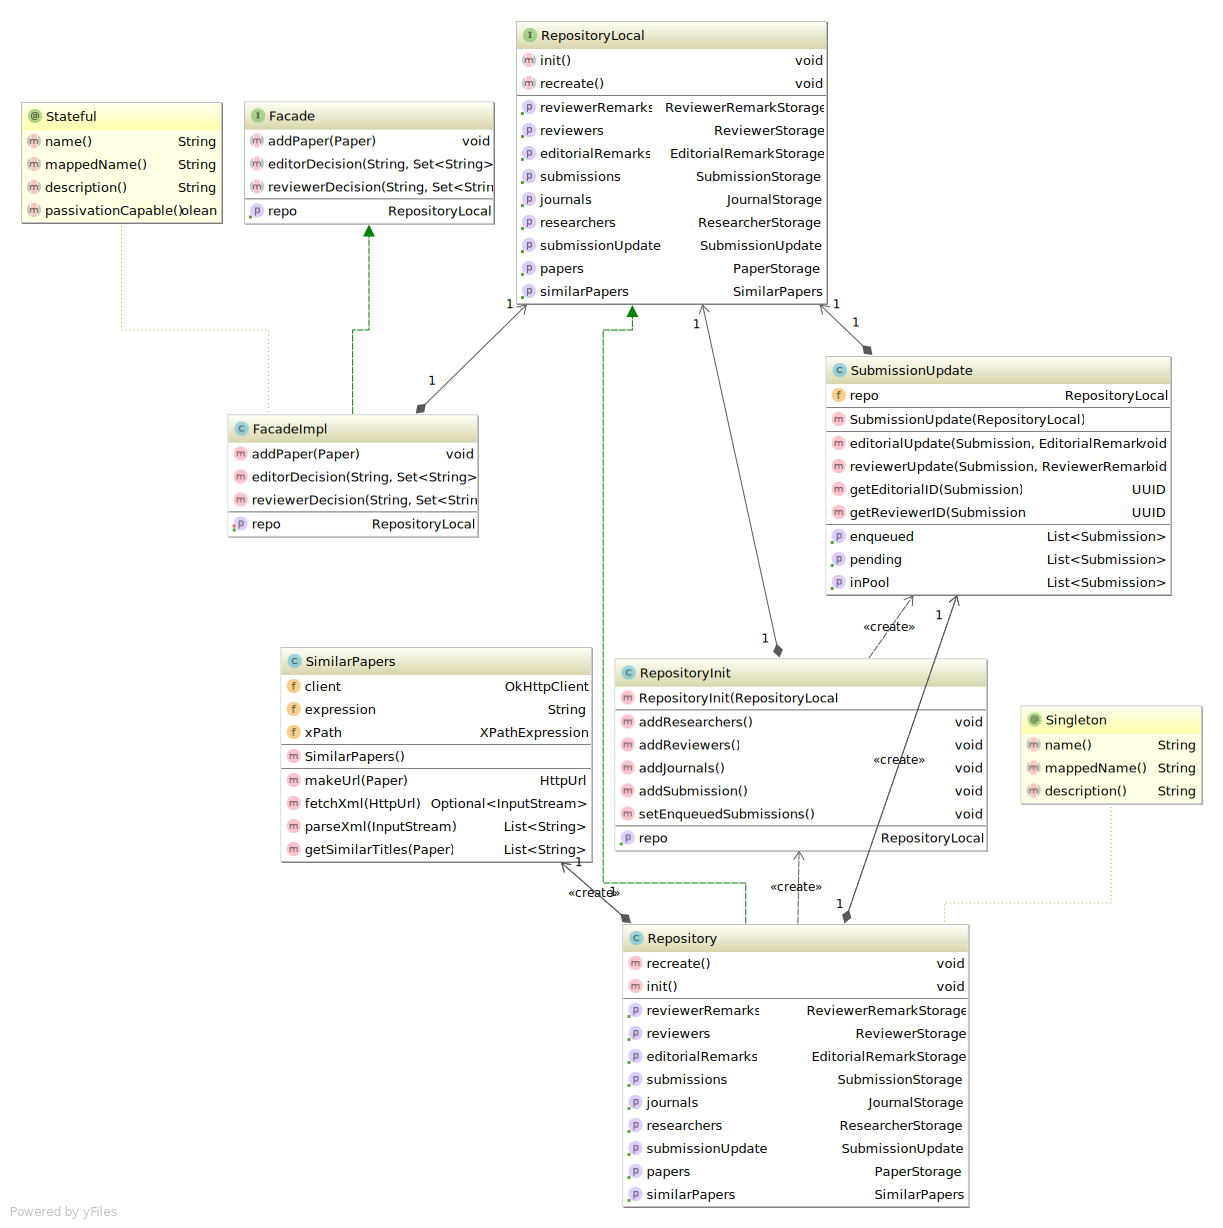
\includegraphics[width=\textwidth]{diagram2.pdf}
\caption{}
\end{figure}

На рисунке \ref{fig:mapper} показана диаграмма классов для слоя хранения.

\begin{figure}[H]
\centering
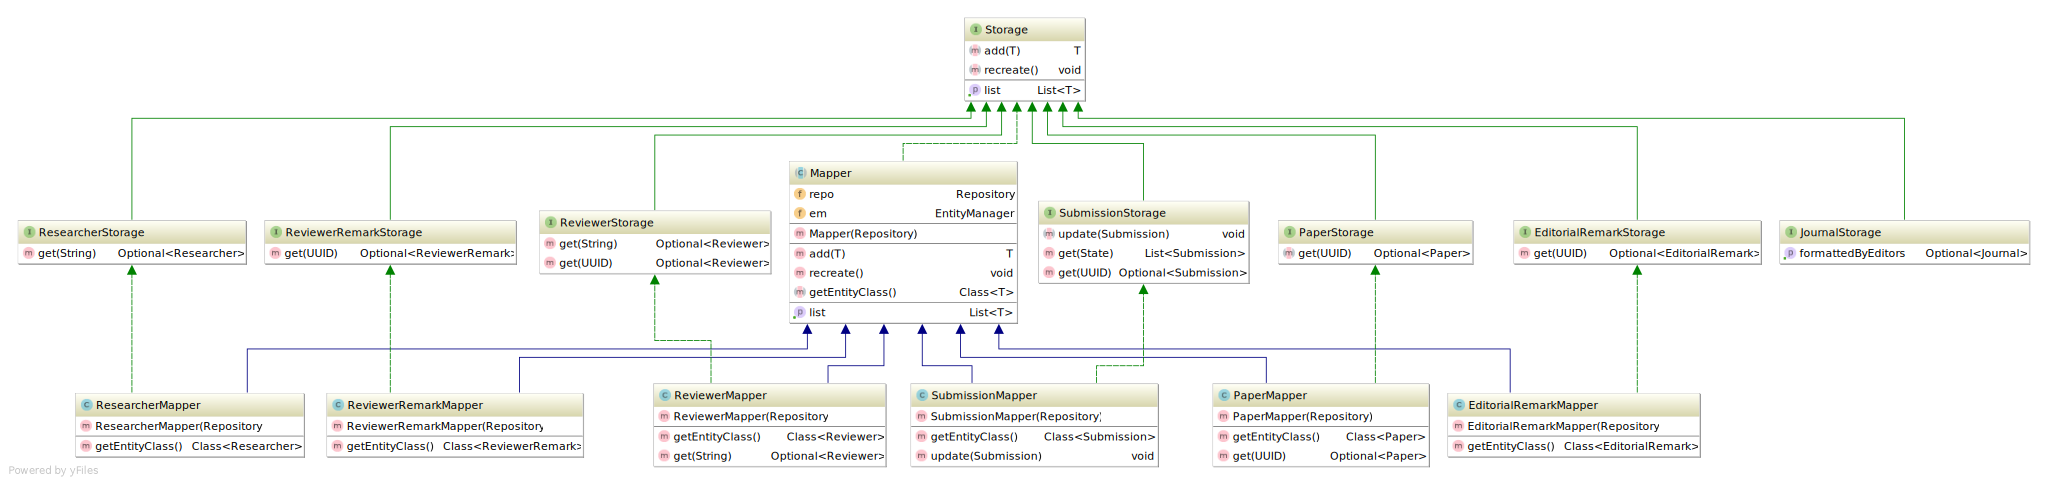
\includegraphics[height=0.97\textheight]{diagram3.pdf}
\caption{}
\label{fig:mapper}
\end{figure}

\subsection{Описание программы}

Было решено, что в приложении будет два bean-а:
\begin{enumerate}
\item Facade - класс для реализации паттерна проектирования <<Фасад>>. Соответствующий Bean было решено сделать @Stateful, чтобы исключить проблемы, связанные с одновременным использованием одного экземпляра класса несколькими клиентами.
\item Repository - класс-репозиторий, содержащий ссылки на объекты-Mapper-ы. Так как все клиенты используют общий набор Mapper-ов, класс Repository был помечен аннотацией @Singleton.
\end{enumerate}

Класс Facade содержит следующие методы:

\begin{itemize}
\item getRepo() - возвращает объект-репозиторий. Внутри класса Facade содержится поле repo, которое автоматически заполняется EJB-контейнером при создании нового экземпляра класса. Для этого поле repo было помечено аннотацией @EJB.
\item addPaper() - добавляет статью в базу данных, и создает для неё новый объект <<Подача>> (Submission).
\item editorDecision(String uuidString, Set<String> params, String remarkText) - для указанной статьи устанавливает решение редактора и добавляет примечание
\item reviewerDecision(String uuidString, Set<String> params, String user, String remarkText) - для указанной статьи устанавливает решение рецензента и добавляет примечание
\end{itemize}

Для реализации Web-интерфейса была использована библиотека Spark, которая в свою очередь основана на API Servlet. Логика веб-интерфейса реализована в классе WebUI. В этом классе имеется только один метод, init, в котором устанавливаются обработчики для различных адресов. Для настройки сервера приложений использовался файл web.xml.

ORM реализован с помощью фреймворка Hibernate. Имеется класс Mapper, который осуществляет взаимодействие с EntityManager-ом. Пример получения данных из БД:

\begin{lstlisting}
CriteriaQuery<T> query = em.getCriteriaBuilder().createQuery(getEntityClass());
Root<T> root = query.from(getEntityClass());
query.select(root);
return em.createQuery(query).getResultList();
\end{lstlisting}

\section{Тестирование}
\begin{figure}[H]
\centering
\includegraphics[width=\textwidth]{researcher.png}
\caption{Страница исследователя}
\end{figure}
Тестирование страницы исследователя:
\begin{center}
	\begin{longtable}{|p{0.3\linewidth}|p{0.3\linewidth}|p{0.3\linewidth}|}
		\hline
		\textbf{Вариант использования} & \textbf{Ожидаемый результат}&
		\textbf{Фактический результат}\\
		\hline
		Выбор исследователя из списка и нажатие кнопки отправить & Выбранный пользователь становится текущим & Над полем выбора пользователя появляется строчка: <<Current researcher is: Имя исследователя>> \\
		\hline
		Заполнение полей Title, Abstract и Content и нажатие кнопки <<Отправить>> & В списке статей появится новая статья & В разделе Submissions появляется новая запись \\
		\hline
	\end{longtable}
\end{center}

\begin{figure}[H]
\centering
\includegraphics[width=\textwidth]{editor.png}
\caption{Страница редактора}
\end{figure}
Тестирование страницы редактора:
\begin{center}
	\begin{longtable}{|p{0.3\linewidth}|p{0.3\linewidth}|p{0.3\linewidth}|}
		\hline
		\textbf{Вариант использования} & \textbf{Ожидаемый результат}&
		\textbf{Фактический результат}\\
		\hline
		Выбор статьи из списка и нажатие кнопки Accept & Статья перейдет в состояние <<Принято>> & Статья исчезает из списка на странице (помечается как просмотренная), на странице исследователя появляется отметка <<Review remark: ACCEPT Note: Сообщение>> \\
		\hline
		Выбор статьи из списка и нажатие кнопки Needs Rework & Статья перейдет в состояние <<Требуется исправление>> & Статья исчезает из списка на странице (помечается как просмотренная), на странице исследователя появляется отметка <<Review remark: NEEDS\_REWORK Note: Сообщение>> \\
		\hline
		Выбор статьи из списка и нажатие кнопки Redirect to another journal & Статья перейдет в состояние <<Статья для другого журнала>> & Статья исчезает из списка на странице (помечается как просмотренная), на странице исследователя появляется отметка <<Review remark: REDIRECT Note: Сообщение>> \\
		\hline
	\end{longtable}
\end{center}

\begin{figure}[H]
\centering
\includegraphics[width=\textwidth]{reviewer.png}
\caption{Страница рецензента}
\end{figure}
Тестирование страницы рецензента:
\begin{center}
	\begin{longtable}{|p{0.3\linewidth}|p{0.3\linewidth}|p{0.3\linewidth}|}
		\hline
		\textbf{Вариант использования} & \textbf{Ожидаемый результат}&
		\textbf{Фактический результат}\\
		\hline
		Выбор статьи из списка и нажатие кнопки Accept & Статья перейдет в состояние <<Готова для печати (In pool)>> для последующей отправки в журнал & Статья исчезает из списка на странице (помечается как просмотренная), на странице исследователя появляется отметка <<Review remark: ACCEPT Note: Сообщение>>, статья доступна для выгрузки в журнал \\
		\hline
		Выбор статьи из списка и нажатие кнопки Neutral & Статья перейдет в состояние <<Готова для печати (In pool)>> для последующей отправки в журнал & Статья исчезает из списка на странице (помечается как просмотренная), на странице исследователя появляется отметка <<Review remark: NEUTRAL Note: Сообщение>>, статья доступна для выгрузки в журнал \\
		\hline
		Выбор статьи из списка и нажатие кнопки Reject & Статья перейдет в состояние <<Отклонена (Rejected)>> & Статья исчезает из списка на странице (помечается как просмотренная), на странице исследователя появляется отметка <<Review remark: REJECTED Note: Сообщение>> \\
		\hline
	\end{longtable}
\end{center}

\subsection{Инструкция системного администратора}

Исходный код веб-приложения доступен по адресу:

\url{https://github.com/h31/SoftwareArchitecture}

Для корректной работы проекта требуется установить следующее ПО:

\begin{itemize}
\item Пакет Java Runtime Environment 8
\item Сервер приложений WildFly 10
\end{itemize}

Для сборки проекта необходимо выполнить команду ./gradlew war:

\begin{lstlisting}
$ ./gradlew war
:clean
:compileJava
:processResources
:classes
:war

BUILD SUCCESSFUL

Total time: 0.946 secs
\end{lstlisting}

Собранный war-файл доступен по следующему пути: build/libs/\\SoftwareArchitecture.war

После сборки необходимо установить и настроить WildFly. С помощью скрипта add-user.sh добавим пользователя-администратора:

\begin{lstlisting}
artyom@artyom-MSI:~/Tools/wildfly-10.1.0.Final$ bin/add-user.sh 

What type of user do you wish to add? 
 a) Management User (mgmt-users.properties) 
 b) Application User (application-users.properties)
(a): 

Enter the details of the new user to add.
Using realm 'ManagementRealm' as discovered from the existing property files.
Username : user
Password recommendations are listed below. To modify these restrictions edit the add-user.properties configuration file.
 - The password should be different from the username
 - The password should not be one of the following restricted values {root, admin, administrator}
 - The password should contain at least 8 characters, 1 alphabetic character(s), 1 digit(s), 1 non-alphanumeric symbol(s)
Password : 
WFLYDM0099: Password should have at least 8 characters!
Are you sure you want to use the password entered yes/no? yes
Re-enter Password : 
What groups do you want this user to belong to? (Please enter a comma separated list, or leave blank for none)[  ]: 
About to add user 'user' for realm 'ManagementRealm'
Is this correct yes/no? yes
Added user 'user' to file '/home/artyom/Tools/wildfly-10.1.0.Final/standalone/configuration/mgmt-users.properties'
Added user 'user' to file '/home/artyom/Tools/wildfly-10.1.0.Final/domain/configuration/mgmt-users.properties'
Added user 'user' with groups  to file '/home/artyom/Tools/wildfly-10.1.0.Final/standalone/configuration/mgmt-groups.properties'
Added user 'user' with groups  to file '/home/artyom/Tools/wildfly-10.1.0.Final/domain/configuration/mgmt-groups.properties'
Is this new user going to be used for one AS process to connect to another AS process? 
e.g. for a slave host controller connecting to the master or for a Remoting connection for server to server EJB calls.
yes/no? no
\end{lstlisting}

После добавления пользователя можно запустить сам сервер приложений с помощью скрипта standalone.sh

\begin{lstlisting}
artyom@artyom-MSI:~/Tools/wildfly-10.1.0.Final$ bin/standalone.sh
=========================================================================

  JBoss Bootstrap Environment

  JBOSS_HOME: /home/artyom/Tools/wildfly-10.1.0.Final

  JAVA: /usr/lib/jvm/java-8-oracle/bin/java

  JAVA_OPTS:  -server -Xms64m -Xmx512m -XX:MetaspaceSize=96M -XX:MaxMetaspaceSize=256m -Djava.net.preferIPv4Stack=true -Djboss.modules.system.pkgs=org.jboss.byteman -Djava.awt.headless=true

=========================================================================
...
13:13:05,239 INFO  [org.jboss.as] (Controller Boot Thread) WFLYSRV0060: Http management interface listening on http://127.0.0.1:9990/management
13:13:05,239 INFO  [org.jboss.as] (Controller Boot Thread) WFLYSRV0051: Admin console listening on http://127.0.0.1:9990
\end{lstlisting}

WildFly выведет на консоль адрес страницы для управления сервером приложения. Зайдем на неё с помощью браузера:

\begin{figure}[H]
\centering
\includegraphics[width=\textwidth]{wildfly.png}
\caption{}
\end{figure}

В пункте Deployment выберем пункт Start:

\begin{figure}[H]
\centering
\includegraphics[width=\textwidth]{wildfly2.png}
\caption{}
\end{figure}

Далее необходимо нажать на кнопку Add. Откроется окно, где нужно выбрать собранный war-файл:

\begin{figure}[H]
\centering
\includegraphics[width=\textwidth]{wildfly3.png}
\caption{}
\end{figure}

Развернутое приложение доступно по следующему адресу: \\ \url{http://127.0.0.1:8080/SoftwareArchitecture/}

\section{Инструкция пользователя}

По умолчанию веб-сайт доступен по адресу

\url{http://127.0.0.1:8080/SoftwareArchitecture/}.

Ниже приведен снимок экрана с главной страницей веб-приложения.

\begin{figure}[H]
\centering
\includegraphics[width=\textwidth]{page.png}
\caption{}
\end{figure}

\subsection{Инструкция исследователя}

\begin{figure}[H]
\centering
\includegraphics[width=\textwidth]{researcher.png}
\caption{Страница исследователя}
\end{figure}

Если пользователь - исследователь, ему необходимо пройти в раздел Researcher по соответствующей ссылке. Для дальнейшей работы пользователю необходимо аутентифицироваться. В верхней части страницы в выпадающем списке необходимо выбрать нужного пользователя и нажать кнопку <<Отправить>>.

Следующий этап - заполнить на странице поля <<Заголовок (Title)>>, <<Реферат (Abstract)>> и <<Содержимое статьи (Content)>>. После заполнения всех полей следует нажать кнопку <<Отправить>>.

После отправки статьи пользователь может увидеть её в списке в верхней части экрана.

\subsection{Инструкция редактора}

\begin{figure}[H]
\centering
\includegraphics[width=\textwidth]{editor.png}
\caption{Страница редактора}
\end{figure}

Если пользователь - редактор, ему необходимо пройти в раздел Editor по соответствующей ссылке. В этом разделе в верхней части страницы перечислены новые (ещё не просмотренные) статьи. В списке для каждой статьи указан её заголовок, реферат и непосредственно содержимое.

Если редактор решает, что статья соответствует тематике журнала и удовлетворяет правилам оформления, ему нужно нажать кнопку <<Accept>>. Странице обновляется, и статья пропадает из списка не просмотренных статей. Если редактор отказывает в приеме статьи по причине недоработок в статье (например, проблемах с форматированием), ему необходимо указать список замечаний, который будет передан автору, и нажать кнопку <<Suggest rework>>. Если редактор отказывает в приеме по причине несоответствия тематике журнала, он указывает список замечаний и нажимает кнопку <<Redirect to another journal>>.

\subsection{Инструкция рецензента}

\begin{figure}[H]
\centering
\includegraphics[width=\textwidth]{reviewer.png}
\caption{Страница рецензента}
\end{figure}

Если пользователь - рецензент, ему необходимо пройти в раздел Reviewer по соответствующей ссылке. В верхней части страницы в выпадающем списке необходимо выбрать нужного пользователя и нажать кнопку <<Отправить>>. Под блоком аутентификации на странице перечислены новые (ещё не просмотренные) статьи. В списке для каждой статьи указан её заголовок, реферат и непосредственно содержимое.

Если рецензент одобряет статью для публикации (Accept), то ему нужно нажать кнопку <<Accept>>. Если рецензент имеет замечания к статье, но допускает её для публикации (Neutral), он должен нажать кнопку <<Neutral>>. Если рецензент имеет замечания к статье и не допускает её для публикации (Reject), он должен нажать кнопку <<Reject>>. Во всех случаях в текстовом поле около кнопок необходимо указать рецензию. После нажатия одной из кнопок статья отмечается в системе как принятая и исчезает из списка.

\section{Выводы}
В рамках данного курса были изучены принципы разработки программного обеспечения для распределенных вычислительных систем. Были изучены технологии EJB (Enterprise Java Beans) и JPA (Java Persistence API). В соответствии с этими принципами и с использованием перечисленных технологий было разработано приложение - информационная система для научного журнала.

В качестве сервера приложений использовался WildFly 10, в качестве ORM - Hibernate 5. Для хранения данных использовалась СУБД PostgreSQL 9.5.

Возможные пути улучшения разработанного приложения:

\begin{itemize}
\item Добавление возможности составления и верстки журнала. При этом возможно появление ещё одной роли - верстальщика. Результат верстки - электронный документ в одном из распространенных форматов (например, PDF).
\item Добавление интерфейса читателя
\end{itemize}

Приложение удовлетворяет требованиям прозрачности, масштабируемости и открытости, во многом благодаря использованию технологий HTML, EJB и JPA.